\chapter{Implementation: Designing CCP Datapaths}
The advantage of the CCP system includes allowing algorithm developers to not concern themselves with deploying their code on different datapaths.
A CCP compatible datapath needs to accurately enforce the congestion control algorithm sent down by the CCP userspace module. Algorithm developers do not need to worry about datapath specific concerns, such as accurately measuring signals and setting the correct sending rate. Furthermore, once a datapath correctly implements support for CCP, this automatically enables support for all CCP algorithms.

In order to implement support for CCP in both QUIC and the Linux Kernel, we designed a CCP datapath API, \libccp, to make the life of the datapath developer easier. This API clearly defines the job of the datapath developer as well as handles CCP specific computation common to all datapaths. This chapter briefly describes the CCP algorithm interface, and then it describes the implementation of \libccp, and how we use \libccp to design a CCP datapath in QUIC.

\section{CCP Algorithm Interface}
At a high level, congestion control algorithms measure and update statistics about the network, every time they receive new information, usually on packet ACK arrivals, in order to decide how fast to send packets. TCP, for example, in its normal operation, keeps increasing the congestion window until seeing a packet loss, upon which it cuts the congestion window in half.
All CCP datapaths must work with the CCP Agent, run in userspace on the same host.
To support the CCP algorithms written, datapaths must calculate aggregate measurements written over certain congestion primitives, and perform actions at the correct time. These actions include setting windows and pacing rates, as well as reporting measurements back up the main CCP agent.
In the Linux kernel, and in QUIC, congestion control decisions are tied to the ACK clock - decisions must be made everytime an ACK arrives, signaling a congestion event.
Another advantage of CCP is that algorithms can take congestion control actions off of the ACK clock, by explicitly defining a slow path and a fast path program.
In the slow path program, written through the CCP API, algorithms respond to reports that are sent up at granularities specified by the fast path.
Fast path programs run in the datapath, per ACK, and send reports up for the slow path programs to respond to.
The CCP API is currently written in Rust, with bindings to Python.  must write two functions in the slow path:
  \begin{itemize}
    \item \texttt{onCreate} - what to do when a flow is created. Users must install some program here, or else they will not get any measurements
    \item \texttt{onReport} - what to do with measurements when reports are received. This may involve some more complicated calculation, such as fast fourier transforms or neural networks.
  \end{itemize}

\subsection{Fast path programs}
Installing a program involves sending down a string, that defines variables, event handlers. These programs use a Scheme-like syntax The variables are aggregated measurements over certain congestion primitives provided by the datapath. The event handlers consist of a condition, and instructions to execute if the condition is true. Event conditions can access the user defined variables, or other special variables, such as time.
Below is an excerpt of the CCP BBR program sent down to the datapath.

%{\footnotesize
\begin{minted}{lisp}
(def
    (acked 0)
    (lost  0)
)
(when true
    (:= acked (+ acked Ack.bytes_acked))
    (:= lost  (+ lost  Ack.lost_pkts_sample))
    (fallthrough)
)
(when (> lost 0)
    (report)
)
\end{minted}

Table~\ref{tab:api} define the operations, primitive congestion signals, and variable scopes supported by the CCP.
\begin{table}
    \label{tab:api}
    \centering
    \begin{tabular}{p{0.35\columnwidth}p{0.5\columnwidth}}
        \hline
        \hline
        \multicolumn{2}{c}{Primitive congestion signals} \\
        \hline
        \hline
        \textbf{Signal} & \textbf{Definition} \\
        \texttt{Ack.bytes\_acked}, \texttt{Ack.packets\_acked} & In-order acknowledged \\
        \texttt{Ack.bytes\_misordered}, \texttt{Ack.packets\_misordered} & Out-of-order acknowledged \\
        \texttt{Ack.ecn\_bytes}, \texttt{Ack.ecn\_packets} & ECN-marked \\
        \texttt{Ack.lost\_pkts\_sample} & Number of lost packets \\
        \texttt{Ack.now} & Datapath time (e.g., wall clock time)\\
        \texttt{Flow.was\_timeout} & Did a timeout occur? \\
        \texttt{Flow.rtt\_sample\_us} & A recent sample RTT \\
        \texttt{Flow.rate\_outgoing} & Outgoing sending rate \\
        \texttt{Flow.rate\_incoming} & Receiver-side receiving rate  \\
        \texttt{Flow.bytes\_in\_flight}, \texttt{Flow.packets\_in\_flight} & Sent but not yet acknowledged \\
        & \\
        \hline
        \hline
        \multicolumn{2}{c}{Operators} \\
        \hline
        \hline
        \textbf{Class} & \textbf{Operations} \\
        Arithmetic & $+, -, *,$~/$,$ EWMA \\
        Assignment & $:=$ \\
        Comparison & $==, <, >$, or, and \\
        Conditionals & If (branching) \\
        & \\
        \hline
        \hline
        \multicolumn{2}{c}{Variable Scopes} \\
        \hline
        \hline
        \textbf{Scope} & \textbf{Description} \\
        \texttt{Ack} & Signals measured per packet \\
        \texttt{Flow} & Signals measured per connection \\
        \texttt{Timer} & Multi-resolution timer that can be zeroed by a call to \texttt{reset} \\
    \end{tabular}
    %\vspace{0.075in}
    \caption{Fast path language: primitive signals, operators, and scopes. As per the CCP API, datapaths must exposes these signals and operators}
\end{table}


\section{Responsibilities of a CCP Datapath}

A CCP datapath must parse and run a program sent down by the CCP agent that represents a congestion control algorithm.
In order to do this accurately, a CCP datapath has three main responsibilities.
  \begin{itemize}
    \item Establish an IPC mechanism.
    \item Correctly enforce congestion windows and pacing rates
    \item Accurately measure the variables defined, and run the program sent by the user everytime new information comes.
  \end{itemize}
First, it must communicate with the CCP agent, that runs on the same host, using some interprocess communication (IPC) mechanism.
The current implementation of the CCP Agent expects that the datapath communicates through a single persistent connection.
Regardless of how many new flows enter, the datapath must be able to send and receive messages about all flows over this single connection.
It must assign flow IDs and uses these IDs to distinguish between flows when serializing and deserializing messages.

In order to accurately enforce the sending patterns of the congestion control algorithm, datapaths should enforce pacing rates and congestion windows separately. This would allow an algorithm to specify a congestion window with a rate cap, in order to prevent bursty transmission.

Third, the datapath must measure congestion signals accurately and report them to the CCP agent at the specified timing patterns.
This involves correctly installing and performing the programs sent down by the CCP agent, which specify how to aggregate and report measurements over the congestion primitives and how to set the congestion window and pacing rate. While the CCP agents turns the user's programs into a serialized set of instructions for the datapath, the datapath must ensure safe execution of the instructions. For the Linux kernel datapath, this involves ensuring that instructions cannot cause a divide by zero that would crash the kernel.


\section{Libccp}

To help add CCP support in various datapaths, we created a shared library in C, named \libccp that provides a reference implementation for the features common to all CCP datapaths: serialization of messages and execution of the program sent down by the userspace agent.
As we built our kernel, QUIC, and mTCP datapaths simultaneously, having one body of shared code prevented reimplementing the same work to multiple datapaths.
This shared library also reduces the responsibilities required by CCP datapaths to provide support for CCP algorithms.
Now datapath developers solely need to focus on (i) \textit{correctly defining primitive congestion signals} and (ii) \textit{correctly exposing mechanisms to set congestion windows and pacing rates}
Specifically, to implement the datapath API, datapaths must provide a set of function pointers, set up IPC with some form compatible with userspace CCP (character device or netlink sockets for kernel datapaths, and unix sockets for userspace datapaths), and fill in the congestion signal primitives everytime new information arrives.
Datpath developers must provide function pointers that do the following:
\begin{enumerate}
    \item Set a congestion window (in bytes)  or pacing rate (either an absolute rate, or relative to current rate) given a flow ID
    \item Provide a notion of time: now, since, and after (in microseconds)
    \item Send a message through the IPC to the userspace CCP agent
\end{enumerate}
Each of these functions takes in a pointer to \ct{struct ccp\_connection}, which contains information for this flow. \ct{ccp\_connection} includes one field for datapath specific state per flow. In the Linux kernel, for example, this is pointer to the \ct{tp\_sock} object, to access congestion state for the correct connection.

In return, \libccp provides two functions that the datapath can call to make userspace CCP algorithms work properly.
\begin{itemize}
    \item \texttt{ccp\_invoke}: After updating the primitive congestion signals on ACKs and timeouts, \texttt{ccp\_invoke} will invoke the program state machine stored inside \libccp. This will run through all of the events in the currently installed program, ending with an optional report to the userspace CCP agent; the events will automatically invoke the function pointers that set the rate or cwnd within the datapath.
    \item \texttt{ccp\_read\_msg}: Upon reading a message from the IPC mechanism, the datapath can call \texttt{ccp\_read\_msg}. 
        Currently, CCP can send down two types of messages: a message that updates the value of a particular variable defined by the fast past program, or a message to install a new fast path program completely. 
        \libccp will deserialize the message to parse both the flow ID and message type from the header, in order to perform the correct update for the correct flow.
\end{itemize}

With the architecture of the \libccp API, adding support into QUIC for supporting CCP was relatively easy.

\section{Current Congestion Control Architecture in QUIC}
As discussed in \dr{related work}, the QUIC already supports pluggable congestion control in userspace. \dr{ref to send algorithm interface}
\begin{figure}[h]
\centering
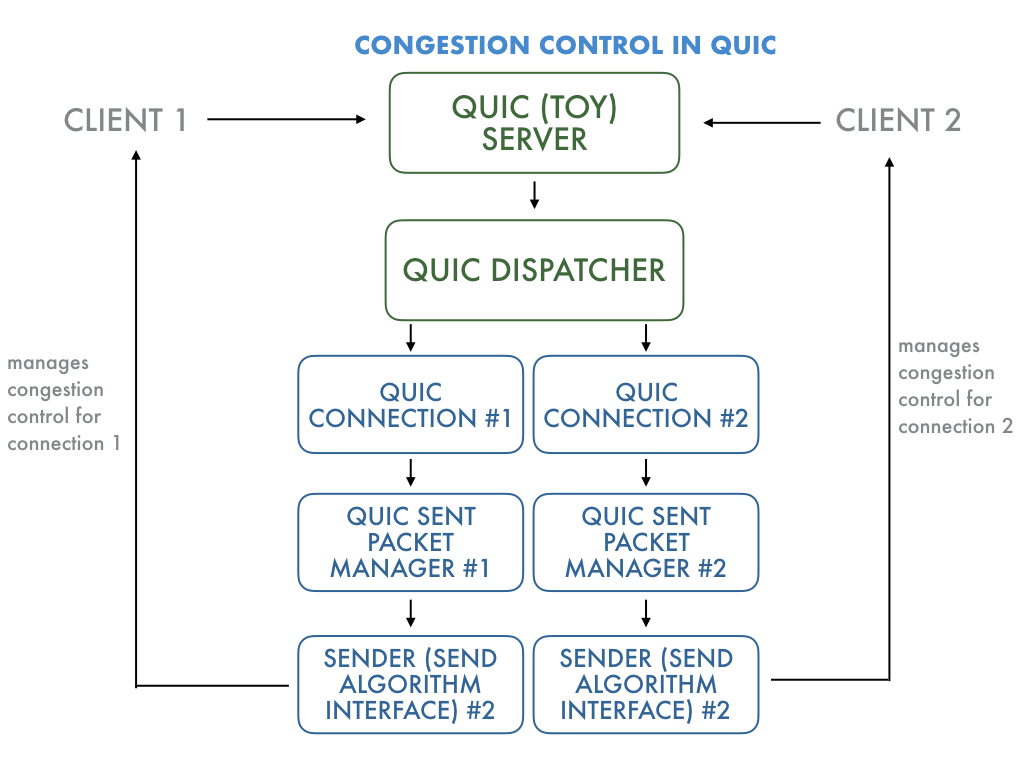
\includegraphics[scale=.45]{implementation/quiccc}
\caption{In QUIC, when the toy server sees a client request, the \ct{SimpleDispatcher} object spawns a new \ct{QuicConnection} object that handles the connection. To manage sending packets, the \ct{QuicConnection} object creates a \ct{QuicSentPacketManager}. The \ct{QuicSentPacketManager} creates a \ct{Sender} object that uses the function callbacks from the \ct{SendAlgorithmInterface} specified as the current congestion control setting.}
\label{fig:quiccc_diagram}
\end{figure}

As Fig~\ref{fig:quiccc_diagram} shows, QUIC uses the \ct{SendAlgorithmInterface} class to allow developers to add in new algorithms.
The \ct{SendAlgorithmInterface} contains most of the features necessary to support a CCP datapath.
The \ct{GetCongestionWindow()} and \ct{PacingRate()} functions allow algorithms to set particular congestion windows and pacing rate.
Pacing is implemented through a separate sender class with a typical token bucket scheme. When deciding whether to send more, the \ct{QuicConnection} object invokes the \ct{CanSend} callback.
This function takes in the number of bytes in flight, and checks whether the congestion window is less, so the sender can send more.
If pacing is enabled and the pacing rate is not 0, the \ct{QuicConnection} checks whether sending should be delayed due to pacing.
Three functions allow senders to measure the congestion signals specified in Table~\ref{tab:api}:
\begin{itemize}
	\item \ct{OnCongestionEvent}: Incoming ACKs or loss event timeouts trigger this function, which provides a vector of acked packets, a vector of lost packets, a boolean indicating if the RTT has been updated, and the prior in flight byte count.
	\item \ct{OnPacketSent}: This callback provides new information on the current number of bytes in flight.
	\item \ct{OnRetransmissionTimeout}: This callback allows senders to take any special actions in the case of timeouts; packets are not counted as lost in the case of timeouts.
\end{itemize}

To implement support for CCP, it is not enough to just implement a sender.
The main requirement for off datapath congestion control is the ability to use an IPC mechanism to communicate between the in datapath sender and the off datapath congestion control.
Each sender object could independently spawn an IPC mechanism and communicate with the CCP agent, but the current implementation does not support this.
As QUIC is another userspace process, each sender could use UDP to communicate with CCP.
However, the current design of CCP requires that the datapath has one persistent connection with the CCP agent, where messages are received and sent regarding all current flows.
Since each sender is an independent object, it only knows about its own flow; some object higher in the hierarchy from Figure~\ref{fig:quiccc_diagram} must control IPC with the CCP agent.

\section{Implementing Libccp API in QUIC}
\subsection{Architecture}
\begin{figure}[h]
\centering
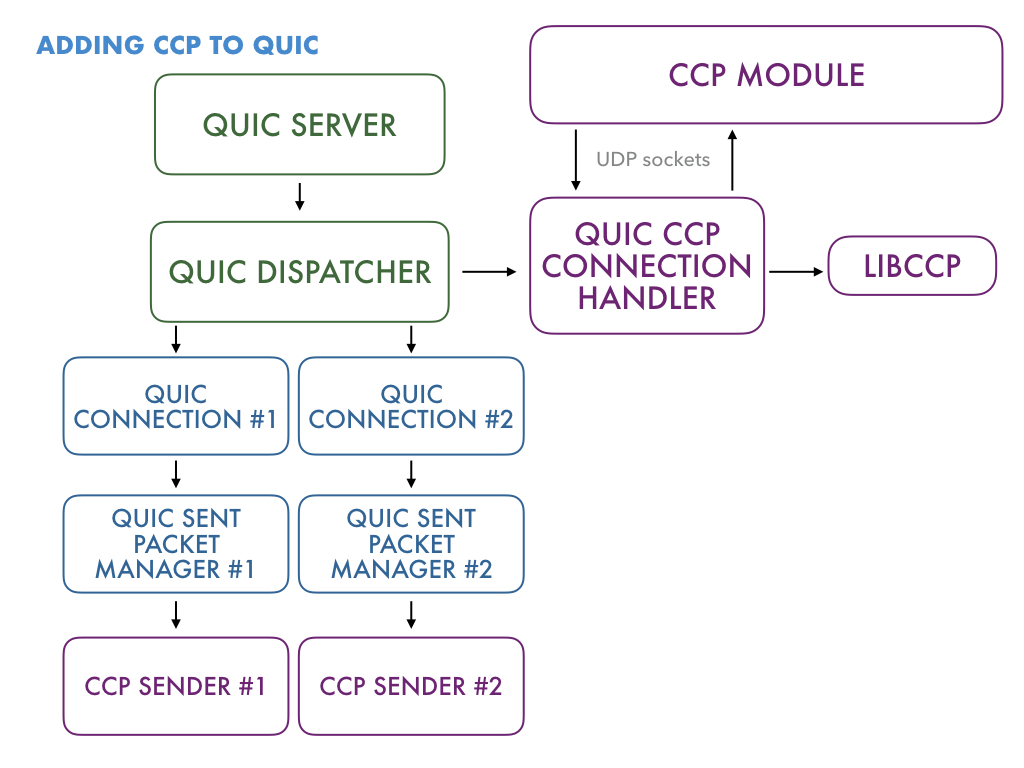
\includegraphics[scale=.45]{implementation/ccpquic_diagram}
\caption{The \ct{QuicCCPConnectionHandler} class implements the \libccp API. It provides the time related functions through the C++ standard library's wall clock time. By passing in the pointer to the specific \ct{QuicConnection} object to a call to \ct{Set\_Congestion\_Window}, the CCP connection handler propagates the instruction down to the specific CCP sender object.}
\label{fig:ccpquic_diagram}
\end{figure}


To implement CCP support in QUIC, we add a new \ct{CCPSender} class that implements the \ct{SendAlgorithmInterface}.
To handle IPC communication with the CCP Agent, we create a new object, the \ct{CCPConnectionHandler}, that uses UDP sockets.
In addition, all the function pointers required by the \libccp API are provided through this class.
The \ct{SimpleDispatcher} owns the \ct{CCPConnectionHandler}; Figure~\ref{fig:ccpquic_diagram} details how the new classes fit into the overall QUIC congestion control architecture.
Upon starting a new connection, the connection handler sets up CCP related state for the flow.
It saves a pointer to the \ct{QuicConnection} object in the \libccp state for this flow.
Later when the fast path program is running and \libccp must set a window or pacing rate for this flow, \libccp calls the set window pointer in the \ct{CCPConnectionHandler} with the \ct{QuicConnection} pointer as argument.

\subsection{Congestion Signal Measurement}\
\begin{table}
    \label{tab:quicsignaldef}
    \centering
    \begin{tabular}{p{0.35\columnwidth}p{0.5\columnwidth}}
        \hline
        \hline
        \multicolumn{2}{c}{Primitive congestion signals} \\
        \hline
        \hline
        \textbf{Signal} & \textbf{Definition} \\
        \texttt{Ack.bytes\_acked}, \texttt{Ack.packets\_acked} & Number of bytes received in order in a call to \ct{OnCongestionEvent} before the first lost packet, from the \ct{AckedPackets} vector passed in as an argument \\
        \texttt{Ack.bytes\_misordered}, \texttt{Ack.packets\_misordered} & Number of bytes received in the \ct{AckedPackets} vector with a sequence number greater than the sequence number of the first lost packet. \\
        \texttt{Ack.lost\_pkts\_sample} & Number of lost packets, i.e. size of the \ct{LostPackets} passed into the \ct{OnCongestionEvent} function. \\
        \texttt{Ack.now} & C++ Standard library wall clock time\\
        \texttt{Flow.was\_timeout} & True when \ct{OnRetransmissionTimeout} is called \\
        \texttt{Flow.rtt\_sample\_us} & The most recent new RTT sample.\\
        \texttt{Flow.rate\_outgoing} & Outgoing sending rate \\
        \texttt{Flow.rate\_incoming} & Receiver-side receiving rate, measured at the sender.  \\
        \texttt{Flow.bytes\_in\_flight}, \texttt{Flow.packets\_in\_flight} & Updated whenever a packet is sent for a new estimate of the number of bytes currently in the pipe. \\
    \end{tabular}
    %\vspace{0.075in}
    \caption{On ACKs, the \ct{CCPSender} uses these definitions to update the calculations of the primitive congestion signals}
\end{table}

Each sender individually measures congestion signals, and calls \ct{ccp\_invoke} to trigger execution of the fastpath program within \libccp.
Table~\ref{tab:quicsignaldef} specifies, within QUIC, how each congestion signal is calculated.
QUIC's notion of acknolwedgements is different from the Linux kernel. The Linux kernel uses the notion of ``sack'' to indicate a packet is lost.
The sender will see acknowledgements for the 3 sequence numbers after the lost packet.
In contrast, QUIC keeps a map of bytes in flight and can explicitly provide information about which sequence numbers are lost, within a block of packets.
\dr{explain this better; explain loss recovery in QUIC better}

\section{Summary of Implementation}
We implement CCP support in the QUIC Toy Server, in the publicly released chromium code base.
The changes, in total, include:
\begin{itemize}
    \item New \ct{CCPSender} that implements the send algorithm interface
    \item Modify \ct{QuicConnection} and \ct{QuicSentPacketManager} classes to allow setting windows for the underlying \ct{CCPSender}
    \item New \ct{QuicCCPConnectionHandler} class
    \item Modify \ct{QuicSimpleDispatcher}, used by the toy server, to spawn a connection handler when starting a new connection
    \item Add \ct{libccp} as a third party library
    \item Command line options when running the toy server to control which congestion control option is set
    \item New congestion window logger class to help with experimenting
\end{itemize}
All the changes are based on top of Chromium commit hash \textbf{dedfa29047}, and comprise of about 1050 new lines of code.
\ct{libccp} is about a 1000-line C library.
 
